\chapter{RESULTADOS E DISCUSSÕES}

O cenário ilustrado na \ref{transmission-at-gnome} evidencia que a adaptação
proposta na interface do Transmission provê maior harmonia com outros
aplicativos da plataforma GNOME.

\begin{figure}[htb]
  \begin{center}
    \caption{\textbf{Transmission no GNOME 3.16}}\label{transmission-at-gnome}
    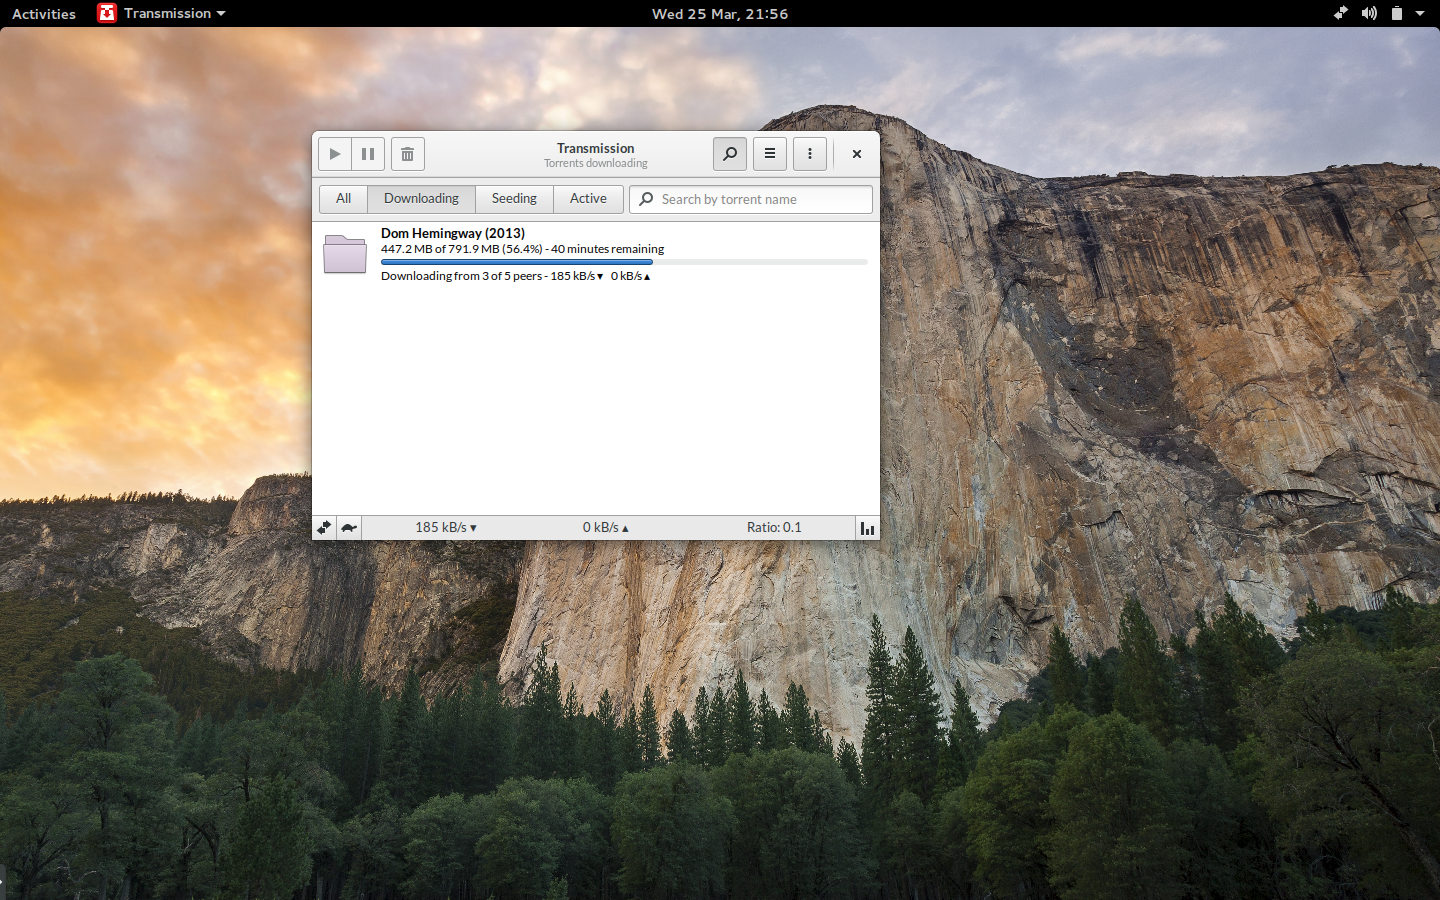
\includegraphics [scale=0.2]{image/transmission-gtk3-main.png}
    \label{transmission-at-gnome}
  \end{center}
\end{figure}

\section{A evolução das aplicações centrais analisadas}

A análise das aplicações centrais do GNOME trouxe resultados efetivos sobre a
transição gráfica e funcional dos principais widgets utilizados pela aplicação.

Um ítem notável foi a redução na utilização de espaço vertical em aplicações
centrais. \citeonline{day2014saving} analisa a redução do uso vertical de espaço
em várias versões do Nautilus e apresenta a seguinte tabela:

\begin{center}
    \begin{tabular}{ | l | l | } 
    \hline
    Versão do Nautilus & Moldura Vertical \\ \hline
    2.22 & 171 pixels \\
    3.0  & 116 pixels \\
    3.6  & 70 pixels \\
    3.12 & 48 pixels \\
    \hline
    \end{tabular}
\end{center}

Observou-se que o fenômeno se repete em todas as aplicações centrais analisadas:

% \begin{figure}[htb]
%   \begin{center}
%     \caption{\textbf{Barra de Cabeçalho - Nautilus}}
%     \includegraphics[width=\textwidth]{image/benchmark/nautilus-headerbar.png}
%     \label{nautilus-headerbar}
%   \end{center}
% \end{figure}

% \begin{figure}[htb]
%   \begin{center}
%     \caption{\textbf{Barra de Cabeçalho - Evince}}
%     \includegraphics[width=\textwidth]{image/benchmark/evince-headerbar.png}
%     \label{evince-headerbar}
%   \end{center}
% \end{figure}

% \begin{figure}[htb]
%   \begin{center}
%     \caption{\textbf{Barra de Cabeçalho - Gedit}}
%     \includegraphics[width=\textwidth]{image/benchmark/gedit-headerbar.png}
%     \label{evince-headerbar}
%   \end{center}
% \end{figure}

\section{Barra de Título}

Um dos elementos de interface mais notáveis é a barra de título. Até então
desenvolvedores tinham pouco ou nenhum controle sobre elas por questões de
compatibilidade de software. Com o surgimento do conceito de `Header Bars', 
as barras de título ganharam  botões, caixas de texto, sliders, etc.

\section{Barra de Filtros}

Mostrar todos os controles de uma só vez torna a aplicação mais díficil de usar.
Portanto é necessário 

\section{Limites Globais de Upload/Download}

\section{Botão Limite de velocidade}

\section{Estísticas da barra de status}
